\large\noindent\fbox{
	\parbox{\textwidth}{
	Utilizzando Matlab, si costruisca una tabella dove, per $h = 10^{-j},j = 1,...,10$ e per la funzione $f(x) = x^{4}$ si riporta il valore di $\theta_{h}(x)$ definito nell'Esercizio 1 in x = 1. Commentare i risultati ottenuti.
	}
}
\begin{flushleft}
	\large \textbf{Soluzione}\\[0.5cm]
	Il seguente codice riguarda la soluzione dell'esercizio 3 con la relativa tabella dei risultati:
	\lstinputlisting[language=Matlab]{Codici/Cap1/Esercizio3.m}
	\begin{center}
		\begin{tabular}{|c|c|}
			\hline
				$h$ & $\theta_{h}(1)$ \\
			\hline
    			\(10^{-1}\) & $4.040000000000002$\\
    			\(10^{-2}\) & $4.000400000000004$\\
    			\(10^{-3}\) & $4.000003999999723$\\
    			\(10^{-4}\) & $4.000000039999230$\\
    			\(10^{-5}\) & $4.000000000403681$\\
    			\(10^{-6}\) & $3.999999999948489$\\
    			\(10^{-7}\) & $4.000000000115023$\\
    			\(10^{-8}\) & $4.000000003445692$\\
    			\(10^{-9}\) & $4.000000108916879$\\
    			\(10^{-10}\) & $4.000000330961484$\\
			\hline
		\end{tabular}
	\end{center}
	Come si nota dalla tabella, la funzione $f(x) = x^{4}$ decresce fino a $ i = 10^{-6}$ dopodiché cresce, come si puo notare anche dal seguente grafico:
	\begin{figure}[H]
	\label{Cap_1_Es_3}
	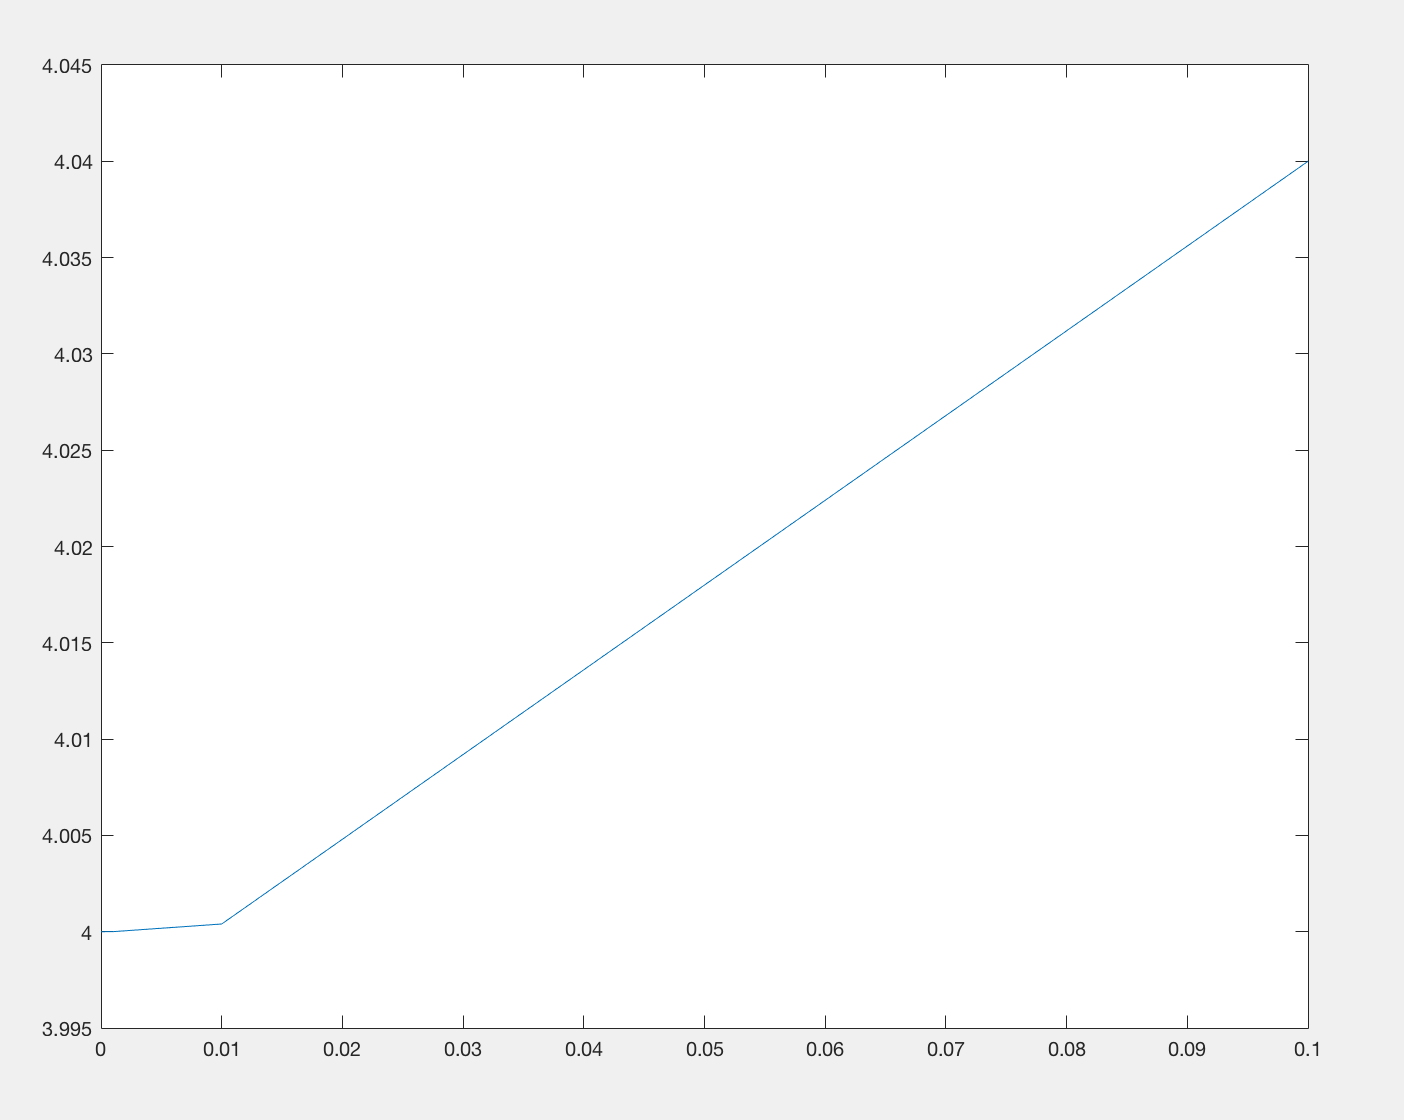
\includegraphics[width=\textwidth]{Codici/Cap1/Es3_Fig}
		\caption{Funzione $\theta_{h}(1)$}
	\end{figure}
\end{flushleft}